\documentclass[10pt]{beamer}
\usepackage{amsmath}
\usepackage{amssymb}
\usepackage{accents}
\usepackage{hyphenat}
\usepackage{multirow}
\usepackage{animate}
% \usepackage[dvipsnames]{xcolor}

\usetheme[progressbar=frametitle]{metropolis}
\setbeamercolor{background canvas}{bg=white}
\usepackage{appendixnumberbeamer}
\usefonttheme[onlymath]{serif}
\usepackage{booktabs}
\usepackage[scale=2]{ccicons}
\usepackage{soul}

\usepackage{pgfplots}
\usepgfplotslibrary{dateplot}

\usepackage{xspace}
\newcommand{\themename}{\textbf{\textsc{metropolis}}\xspace}
\usetikzlibrary{snakes,arrows,mindmap,trees,backgrounds,shapes.geometric,calc}
\tikzset{graphics/.style={inner sep=0,outer sep=0}}
\tikzset{scaleall/.style={scale=#1, transform shape}}
\usepgflibrary{arrows}


\newlength{\bbw}
\newlength{\bbh}
\newcommand{\pcuad}[3][]{
  % First arguments is an optional prefix for the coordinate names

  \setlength{\bbw}{#2}
  \setlength{\bbh}{#3}
  \useasboundingbox(0,0) rectangle (\bbw,\bbh);

  \path(.5\bbw,.5\bbh) coordinate(#1cp);
  \path(\bbw,0)        coordinate(#1se);
  \path(0,0)           coordinate(#1sw);
  \path(0,\bbh)        coordinate(#1nw);
  \path(\bbw,\bbh)     coordinate(#1ne);
 
  
  \path(\bbw,.5\bbh) coordinate(#1ep);
  \path(.5\bbw,0)    coordinate(#1sp);
  \path(.5\bbw,\bbh) coordinate(#1np);
  \path(0,.5\bbh)    coordinate(#1wp);
       
  \path(.75\bbw,.5\bbh) coordinate(#1hr);
  \path(.25\bbw,.5\bbh) coordinate(#1hl);
  \path(.5\bbw,.25\bbh) coordinate(#1vl);
  \path(.5\bbw,.75\bbh) coordinate(#1vu);

  \path(.75\bbw,.75\bbh) coordinate(#1c1);
  \path(.25\bbw,.75\bbh) coordinate(#1c2);
  \path(.25\bbw,.25\bbh) coordinate(#1c3);
  \path(.75\bbw,.25\bbh) coordinate(#1c4);


%  +-----------------------------------------------+
%  |nw                    np                     ne|
%  |                                               |
%  |                                               |
%  |          c2          vu          c1           |
%  |                                               |
%  |                                               |
%  |wp        hl          cp          hr         ep|
%  |                                               |
%  |                                               |
%  |          c3          vl          c4           |
%  |                                               |
%  |                                               |
%  |sw                    sp                     se|
%  +-----------------------------------------------+
}
 
        
\newcommand{\showcuad}[1][]{

   \draw[help lines,xstep=.5,ystep=.5,gray!10] (#1sw) grid (#1ne);
   \draw[help lines,xstep=1,ystep=1,gray]      (#1sw) grid (#1ne);
   %\draw[help lines,xstep=.25,ystep=.25,gray!20] (sw) grid (ne);
   % \draw[help lines,xstep=1,ystep=1,gray] (sw) grid (ne);
   % \foreach \x in {-20,-14.5,...,20} {
   %     \node [anchor=north, gray,yshift=30] at (\x,0) {\tiny \bf \x};
   %     \node [anchor=east,gray,xshift=30] at (0,\x) {\tiny \bf  \x};
   % }
               
    \fill(#1se) circle(.1) node[anchor=south east]{#1se};
    \fill(#1sw) circle(.1) node[anchor=south west]{#1sw};
    \fill(#1ne) circle(.1) node[anchor=north east]{#1ne};
    \fill(#1nw) circle(.1) node[anchor=north west]{#1nw};
                  
    \fill(#1hr) circle(.1) node[above]{#1hr};
    \fill(#1hl) circle(.1) node[above]{#1hl};
    \fill(#1vu) circle(.1) node[above]{#1vu};
    \fill(#1vl) circle(.1) node[above]{#1vl};
                  
    \fill(#1sp) circle(.1) node[anchor=south]{#1sp};
    \fill(#1wp) circle(.1) node[anchor=west] {#1wp};
    \fill(#1np) circle(.1) node[anchor=north]{#1np};
    \fill(#1ep) circle(.1) node[anchor=east] {#1ep};

    \fill(#1cp) circle(.1) node[above]{#1cp};
    \fill(#1c1) circle(.1) node[above]{#1c1};
    \fill(#1c2) circle(.1) node[above]{#1c2};
    \fill(#1c3) circle(.1) node[above]{#1c3}; 
    \fill(#1c4) circle(.1) node[above]{#1c4};

    %\fill[red](cp|-c1) circle(.1) node[anchor=north]{cp|-c1};

}

\newcommand{\ds}{\displaystyle}
\newcommand{\dsum}{\displaystyle \sum}
\newcommand{\uu}[1]{{\boldsymbol #1}}
\newcommand{\ud}{\,\mathrm{d}}
\def\ttau{\uu{\tau}}
\def\bb{\uu{b}}
\def\nb{\uu{n}}
\def\pb{\uu{p}}
\def\wb{\uu{w}}
\def\xb{\uu{x}}
\def\ab{\uu{a}}
\def\mb{\uu{m}}
\def\yb{\uu{y}}
\def\vb{\uu{v}}
\def\fb{\uu{f}}
\def\zb{\uu{z}}
\def\Xb{\uu{X}}
\def\etab{\uu{\eta}}
\def\thetab{\uu{\theta}}
\def\lambdab{\uu{\lambda}}
\def\gammab{\uu{\gamma}}
\def\taub{\uu{\tau}}
\def\varphib{\uu{\varphi}}
\def\Ab{\uu{A}}
\def\Bb{\uu{B}}
\def\Gb{\uu{G}}
\def\Fb{\uu{F}}
\def\Jb{\uu{J}}
\def\Rb{\uu{R}}
\def\Tb{\uu{T}}
\def\rb{\uu{r}}
\def\ab{\uu{a}}
\newcommand{\molar}[1]{\underaccent{\bar}{#1}}
\def\um{\molar{U}}
\def\hm{\molar{H}}
\def\sm{\molar{S}}
\def\am{\molar{A}}
\def\gm{\molar{G}}
\def\hh{\hat{H}}
\def\sh{\hat{S}}
\def\vm{\molar{V}}
\def\cp{C_{\rm P}}
\def\cv{C_{\rm V}}
\def\cps{C_{\rm P}^*}
\def\cvs{C_{\rm V}^*}
\def\wsd{\dot{W}_s}
\def\md{\dot{M}}\newcommand{\pd}[2]{\left(\frac{\partial {#1}}{\partial 
{#2}}\right)}
\newcommand{\tpd}[3]{\left(\frac{\partial {#1}}{\partial {#2}}\right)_{#3}}
\newcommand{\tpdn}[4]{\left(\frac{\partial^{#4} {#1}}{\partial 
{#2}^{#4}}\right)_{#3}}

\definecolor{DUblue}{HTML}{07294D}
\definecolor{DUgold}{HTML}{FFC600}
\definecolor{DUred}{HTML}{9E0B0F}
\definecolor{DUgreen}{HTML}{B7BF10}


\title{Molecular-scale models of Env including MPER-TM}
\date{March 22, 2024}
\author{Cameron F. Abrams and Salsabil Abou-Hatab}
\institute{Drexel University, Department of Chemical and Biological Engineering}
\titlegraphic{\hfill
\includegraphics[height=0.75cm]{drexel-horz-blue.png}}

\begin{document}

\maketitle
\begin{frame}{Outline}
  \setbeamertemplate{section in toc}[sections numbered]
  \tableofcontents[hideallsubsections]
\end{frame}

\section{Ectodomain models based on Tri-FPPR Class 6}
\begin{frame}[fragile]{Models derived from class-6 Tri-FPPR cryo-EM structure}
    % \begin{itemize}
    %     \item ``\textcolor{DUblue}{C6-FT-HHL}'': as-received structure; HR1N unfolded in protomer 3; MPER present in protomer 1 only
    %     \item ``\textcolor{DUblue}{C6-FT-LHL}'': HR1N unfolded in protomers 1 and 3; MPER present in protomer 1 only
    % \end{itemize}
        \begin{center}
            \begin{tabular}{lccl}
                     & \multicolumn{2}{c}{Protomers with} & \\
                name & HR1N unfolded  & MPER & notes\\\hline
                C6-FT-HHL* & 3 & 1 & as-received class-6 structure\\
                C6-FT-LHL & 1,3 & 1 & \\
                C6-FT-LLL & 1,2,3 & 1 & \\
                C6-S1-HHH & -- & 1,2,3 & C$_\alpha$-aln-replication of protomer 1\\
                C6-S1-LLL & 1,2,3 & 1,2,3 & (1) C$_\alpha$-aln-replication of protomer 1\\
                C6-S1-LLLb & 1,2,3 & 1,2,3 & (2) C$_\alpha$-aln-replication of protomer 1\\
                C6-S1-LLLc & 1,2,3 & 1,2,3 & C3-replication of protomer 1\\\hline
            \end{tabular}
        \end{center}
\end{frame}


\begin{frame}[fragile]{MD Simulation General Details}
    \begin{itemize}
        \item All-atom models with all glycan stems retained
        \item All systems built using \href{https://pestifer.readthedocs.io/en/latest/}{pestifer}
        \item Solvated in explicit water (TIP3P)
        \item System sizes 320,000 to 340,000 atoms
        \item NAMD v 2.14 using CHARMM-FF v36
        \item Production MD: NPT (310 K, 1 bar) for 200 ns (100,000,000 time-steps)
        \item Observables:
        \begin{itemize}
            \item opening angles measured via protomer alignment (on gp120 and gp41 separately)
            \item HR1N alpha helicity (not shown in this talk)
            \item $\alpha_9$ tilt angles (not shown in this talk)
            \item snapshots
        \end{itemize}
    \end{itemize}
\end{frame}


\begin{frame}[fragile]{C6-FT-HHL (as-received Tri-FPPR class 6 cryo-EM model)}
    \begin{center}
        \begin{minipage}{0.47\textwidth}
            \begin{center}
                gp120 alignment\\
                \includegraphics[width=\textwidth]{/home/cfa/research/hiv/trifppr/class6/C6_FT_HHL/rotation-matrices-gp120.png}
            \end{center}
        \end{minipage}
        \begin{minipage}{0.47\textwidth}
            \begin{center}
                gp41 alignment\\
                \includegraphics[width=\textwidth]{/home/cfa/research/hiv/trifppr/class6/C6_FT_HHL/rotation-matrices-gp41.png}
            \end{center}
        \end{minipage}

        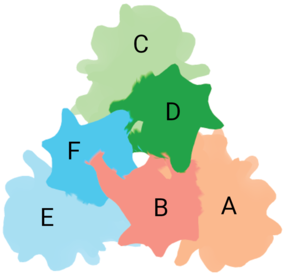
\includegraphics[width=0.16\textwidth]{trimer_paint_bottom_sodroski_smol.png}
        \includegraphics[width=0.19\textwidth]{/home/cfa/research/hiv/trifppr/class6/C6_FT_HHL/images/bottom-view.00000.png}
        \includegraphics[width=0.19\textwidth]{/home/cfa/research/hiv/trifppr/class6/C6_FT_HHL/images/bottom-view.00033.png}
        \includegraphics[width=0.19\textwidth]{/home/cfa/research/hiv/trifppr/class6/C6_FT_HHL/images/bottom-view.00067.png}
        \includegraphics[width=0.19\textwidth]{/home/cfa/research/hiv/trifppr/class6/C6_FT_HHL/images/bottom-view.00100.png}

        Protomer 1 MPER ``flops out'' and binds to protomer 3 gp41
    \end{center}
\end{frame}


\begin{frame}[fragile]{C6-FT-LHL (HR1N unfolded in protomer 1 and 3)}
    \begin{center}
        \begin{minipage}{0.47\textwidth}
            \begin{center}
                gp120 alignment\\
                \includegraphics[width=\textwidth]{/home/cfa/research/hiv/trifppr/class6/C6_FT_LHL/rotation-matrices-gp120.png}
            \end{center}
        \end{minipage}
        \begin{minipage}{0.47\textwidth}
            \begin{center}
                gp41 alignment\\
                \includegraphics[width=\textwidth]{/home/cfa/research/hiv/trifppr/class6/C6_FT_LHL/rotation-matrices-gp41.png}
            \end{center}
        \end{minipage}

        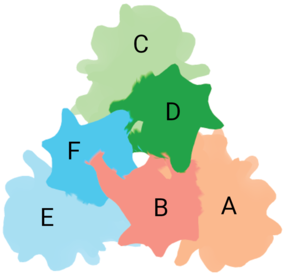
\includegraphics[width=0.16\textwidth]{trimer_paint_bottom_sodroski_smol.png}
        \includegraphics[width=0.19\textwidth]{/home/cfa/research/hiv/trifppr/class6/C6_FT_LHL/images/bottom-view.00000.png}
        \includegraphics[width=0.19\textwidth]{/home/cfa/research/hiv/trifppr/class6/C6_FT_LHL/images/bottom-view.00033.png}
        \includegraphics[width=0.19\textwidth]{/home/cfa/research/hiv/trifppr/class6/C6_FT_LHL/images/bottom-view.00067.png}
        \includegraphics[width=0.19\textwidth]{/home/cfa/research/hiv/trifppr/class6/C6_FT_LHL/images/bottom-view.00099.png}

        Protomer 1 $\alpha$9 and MPER become one helix 
    \end{center}
\end{frame}


\begin{frame}[fragile]{C6-FT-LLL (HR1N unfolded in all protomers)}
    \begin{center}
        \begin{minipage}{0.47\textwidth}
            \begin{center}
                gp120 alignment\\
                \includegraphics[width=\textwidth]{/home/cfa/research/hiv/trifppr/class6/C6_FT_LLL/rotation-matrices-gp120.png}
            \end{center}
        \end{minipage}
        \begin{minipage}{0.47\textwidth}
            \begin{center}
                gp41 alignment\\
                \includegraphics[width=\textwidth]{/home/cfa/research/hiv/trifppr/class6/C6_FT_LLL/rotation-matrices-gp41.png}
            \end{center}
        \end{minipage}

        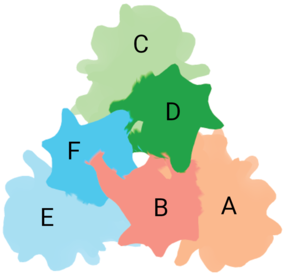
\includegraphics[width=0.16\textwidth]{trimer_paint_bottom_sodroski_smol.png}
        \includegraphics[width=0.19\textwidth]{/home/cfa/research/hiv/trifppr/class6/C6_FT_LLL/images/bottom-view.00000.png}
        \includegraphics[width=0.19\textwidth]{/home/cfa/research/hiv/trifppr/class6/C6_FT_LLL/images/bottom-view.00033.png}
        \includegraphics[width=0.19\textwidth]{/home/cfa/research/hiv/trifppr/class6/C6_FT_LLL/images/bottom-view.00067.png}
        \includegraphics[width=0.19\textwidth]{/home/cfa/research/hiv/trifppr/class6/C6_FT_LLL/images/bottom-view.00099.png}

        Protomer 1 MPER remains relatively stable
    \end{center}
\end{frame}


\begin{frame}[fragile]{C6-S1-HHH (Protomer 1 replicated onto 2, 3)}
    \begin{center}
        \begin{minipage}{0.47\textwidth}
            \begin{center}
                gp120 alignment\\
                \includegraphics[width=\textwidth]{/home/cfa/research/hiv/trifppr/class6/C6_S1_HHH/rotation-matrices-gp120.png}
            \end{center}
        \end{minipage}
        \begin{minipage}{0.47\textwidth}
            \begin{center}
                gp41 alignment\\
                \includegraphics[width=\textwidth]{/home/cfa/research/hiv/trifppr/class6/C6_S1_HHH/rotation-matrices-gp41.png}
            \end{center}
        \end{minipage}

        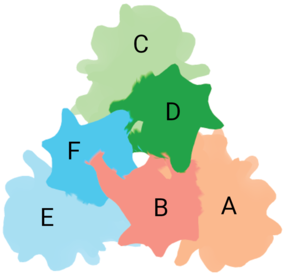
\includegraphics[width=0.16\textwidth]{trimer_paint_bottom_sodroski_smol.png}
        \raisebox{0.5cm}{
\includegraphics[width=0.08\textwidth]{rotate1.png}}
        \includegraphics[width=0.16\textwidth]{/home/cfa/research/hiv/trifppr/class6/C6_S1_HHH/images/side-view.00000.png}
        \includegraphics[width=0.16\textwidth]{/home/cfa/research/hiv/trifppr/class6/C6_S1_HHH/images/side-view.00033.png}
        \includegraphics[width=0.16\textwidth]{/home/cfa/research/hiv/trifppr/class6/C6_S1_HHH/images/side-view.00067.png}
        \includegraphics[width=0.16\textwidth]{/home/cfa/research/hiv/trifppr/class6/C6_S1_HHH/images/side-view.00099.png}

        MPERs move a little
    \end{center}
\end{frame}


\begin{frame}[fragile]{C6-S1-LLL {\tiny (Protomer 1, unfolded HR1N, replicated onto 2, 3)}}
    \begin{center}
        \begin{minipage}{0.47\textwidth}
            \begin{center}
                gp120 alignment\\
                \includegraphics[width=\textwidth]{/home/cfa/research/hiv/trifppr/class6/C6_S1_LLL/rotation-matrices-gp120.png}
            \end{center}
        \end{minipage}
        \begin{minipage}{0.47\textwidth}
            \begin{center}
                gp41 alignment\\
                \includegraphics[width=\textwidth]{/home/cfa/research/hiv/trifppr/class6/C6_S1_LLL/rotation-matrices-gp41.png}
            \end{center}
        \end{minipage}

        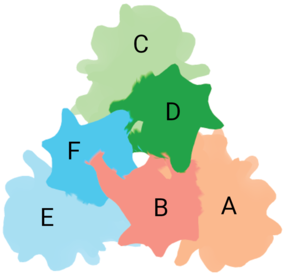
\includegraphics[width=0.16\textwidth]{trimer_paint_bottom_sodroski_smol.png}
        % \raisebox{0.5cm}{
\includegraphics[width=0.08\textwidth]{rotate1.png}}
        \includegraphics[width=0.19\textwidth]{/home/cfa/research/hiv/trifppr/class6/C6_S1_LLL/images/bottom-view.00000.png}
        \includegraphics[width=0.19\textwidth]{/home/cfa/research/hiv/trifppr/class6/C6_S1_LLL/images/bottom-view.00033.png}
        \includegraphics[width=0.19\textwidth]{/home/cfa/research/hiv/trifppr/class6/C6_S1_LLL/images/bottom-view.00067.png}
        \includegraphics[width=0.19\textwidth]{/home/cfa/research/hiv/trifppr/class6/C6_S1_LLL/images/bottom-view.00099.png}

        gp41s become asymmetric
    \end{center}
\end{frame}


\begin{frame}[fragile]{C6-S1-LLLb {\tiny (Protomer 1, unfolded HR1N, replicated onto 2, 3; second replica)}}
    \begin{center}
        \begin{minipage}{0.47\textwidth}
            \begin{center}
                gp120 alignment\\
                \includegraphics[width=\textwidth]{/home/cfa/research/hiv/trifppr/class6/C6_S1_LLLb/rotation-matrices-gp120.png}
            \end{center}
        \end{minipage}
        \begin{minipage}{0.47\textwidth}
            \begin{center}
                gp41 alignment\\
                \includegraphics[width=\textwidth]{/home/cfa/research/hiv/trifppr/class6/C6_S1_LLLb/rotation-matrices-gp41.png}
            \end{center}
        \end{minipage}

        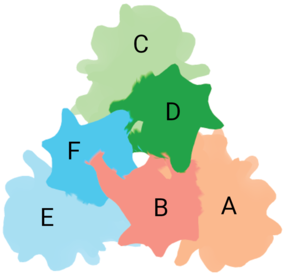
\includegraphics[width=0.16\textwidth]{trimer_paint_bottom_sodroski_smol.png}
        % \raisebox{0.5cm}{
\includegraphics[width=0.08\textwidth]{rotate1.png}}
        \includegraphics[width=0.19\textwidth]{/home/cfa/research/hiv/trifppr/class6/C6_S1_LLLb/images/bottom-view.00000.png}
        \includegraphics[width=0.19\textwidth]{/home/cfa/research/hiv/trifppr/class6/C6_S1_LLLb/images/bottom-view.00033.png}
        \includegraphics[width=0.19\textwidth]{/home/cfa/research/hiv/trifppr/class6/C6_S1_LLLb/images/bottom-view.00067.png}
        \includegraphics[width=0.19\textwidth]{/home/cfa/research/hiv/trifppr/class6/C6_S1_LLLb/images/bottom-view.00099.png}

        % gp41s become asymmetric
    \end{center}
\end{frame}


\begin{frame}[fragile]{C6-S1-LLLc {\tiny (Protomer 1, unfolded HR1N, replicated onto 2, 3; third replica)}}
    \begin{center}
        \begin{minipage}{0.47\textwidth}
            \begin{center}
                gp120 alignment\\
                \includegraphics[width=\textwidth]{/home/cfa/research/hiv/trifppr/class6/C6_S1_LLLc/rotation-matrices-gp120.png}
            \end{center}
        \end{minipage}
        \begin{minipage}{0.47\textwidth}
            \begin{center}
                gp41 alignment\\
                \includegraphics[width=\textwidth]{/home/cfa/research/hiv/trifppr/class6/C6_S1_LLLc/rotation-matrices-gp41.png}
            \end{center}
        \end{minipage}

        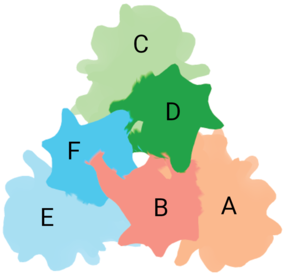
\includegraphics[width=0.16\textwidth]{trimer_paint_bottom_sodroski_smol.png}
        % \raisebox{0.5cm}{
\includegraphics[width=0.08\textwidth]{rotate1.png}}
        \includegraphics[width=0.19\textwidth]{/home/cfa/research/hiv/trifppr/class6/C6_S1_LLLc/images/bottom-view.00000.png}
        \includegraphics[width=0.19\textwidth]{/home/cfa/research/hiv/trifppr/class6/C6_S1_LLLc/images/bottom-view.00033.png}
        \includegraphics[width=0.19\textwidth]{/home/cfa/research/hiv/trifppr/class6/C6_S1_LLLc/images/bottom-view.00067.png}
        \includegraphics[width=0.19\textwidth]{/home/cfa/research/hiv/trifppr/class6/C6_S1_LLLc/images/bottom-view.00099.png}

        % gp41s become asymmetric
    \end{center}
\end{frame}


\begin{frame}[fragile]{SOSIP (State 2) + MPER, aligned on Class-6 Tri-FPPR}

    \includegraphics[width=0.16\textwidth]{ppt/media/image5.png}
    \includegraphics[width=0.16\textwidth]{ppt/media/image6.png}
    \includegraphics[width=0.16\textwidth]{ppt/media/image7.png}
    \includegraphics[width=0.16\textwidth]{ppt/media/image8.png}
    \includegraphics[width=0.16\textwidth]{ppt/media/image9.png}
    \includegraphics[width=0.16\textwidth]{ppt/media/image11.png}

    \includegraphics[width=0.16\textwidth]{ppt/media/image1.png}
    \includegraphics[width=0.16\textwidth]{ppt/media/image2.png}
    \includegraphics[width=0.16\textwidth]{ppt/media/image3.png}
    \includegraphics[width=0.16\textwidth]{ppt/media/image4.png}
    \includegraphics[width=0.16\textwidth]{ppt/media/image10.png}
    \includegraphics[width=0.16\textwidth]{ppt/media/image12.png}

\end{frame}



\section{Membrane-anchored SOSIP-MPER-TM models}
\begin{frame}[fragile]{Models derived from SOSIP Envs and NMR MPER-TM trimers}
    % \begin{itemize}
    %     \item ``\textcolor{DUblue}{C6-FT-HHL}'': as-received structure; HR1N unfolded in protomer 3; MPER present in protomer 1 only
    %     \item ``\textcolor{DUblue}{C6-FT-LHL}'': HR1N unfolded in protomers 1 and 3; MPER present in protomer 1 only
    % \end{itemize}
        \begin{center}
            \begin{itemize}
                \item SOSIPs used are 4zmj (state 2) and 5vn3
                \item all ligands removed, engineered mutations reverted to WT 
                \item gp41's grown out to 687 and then ligated onto MPER-TM 6e8w
                \item Relaxed via MD with TM's held in place
                \item Currently investigating membrane embeddings (z-position of midplane)
            \end{itemize}
        \end{center}
\end{frame}


\begin{frame}[fragile]{Models derived from SOSIP Envs and NMR MPER-TM trimers}
    \begin{center}
        \begin{minipage}{0.47\textwidth}
            \begin{center}
                4zmj (state 2)\\
                \includegraphics[width=\textwidth]{4zmj-mper-tm-example.png}
            \end{center}
        \end{minipage}
        \begin{minipage}{0.47\textwidth}
            \begin{center}
                5vn3 (state 3)\\
                \includegraphics[width=\textwidth]{5vn3-mper-tm-update-1.png}
            \end{center}
        \end{minipage}
        \textcolor{red!80!black}{$\alpha_9$}; 
        \textcolor{yellow!80!black}{MPER};
        \textcolor{blue!80!black}{TM-Lys/Arg};
        \textcolor{orange!90!black}{TM};
        \textcolor{green!80!black}{DOPC}:\textcolor{pink!90!black}{CHOL} (1:1)
\end{center}
\end{frame}



\section{Conclusions}
\begin{frame}[fragile]{Conclusions}
    \begin{itemize}
        \item Tri-FPPR model MD Simulations:
        \begin{itemize}
            \item Single-MPER trimers show poor packing of MPER
            \item Asymmetric trimers remain asymmetric
            \item Unfolding all HR1N's can reduce trimer asymmetry
        \end{itemize}
        \item Membrane-anchored SOSIP-MPER-TM models
        \begin{itemize}
            \item Some ambiguities with membrane embedding need addressing
        \end{itemize}
    \end{itemize}
\end{frame}



\section{Upcoming}
\begin{frame}[fragile]{Upcoming Plans}
    \begin{itemize}
        \item Target models:
        \begin{itemize}
            \item membrane-embedded Tri-FPPR-TM (various configurations of HR1N)
            \item membrane-embedded state-3 SOSIP(5vn3)-MPER-TM(6e8w) (all engineered mutations reverted)
            \item membrane-embedded state-2 SOSIP(4zmj)-MPER-TM(6e8w) (all engineered mutations reverted)
        \end{itemize}
        \item Big questions
        \begin{itemize}
            \item {\bf How do MPERs pack with interprotomer contacts to both gp120 and gp41?}
            \item {\bf How is MPER-TM embedded in membrane in context of ectodomain?}
        \end{itemize}
    \end{itemize}
\end{frame}



\begin{frame}[fragile]{Acknowledgments}
    \begin{center}
        \begin{minipage}[t][.6\textheight]{0.45\textwidth}
            \textcolor{DUred}{\bf Dana Farber Cancer Institute}
            \begin{itemize}
                \item[] Shijian Zhang
                \item[] Zhiqing Zhang
                \item[] Saumya Anang
                \item[] Hanh Nguyen
                \item[] Joe Sodroski
            \end{itemize}
        \end{minipage}\hfill
        \begin{minipage}[t][.6\textheight]{0.45\textwidth}
            \textcolor{DUred}{\bf Yale University}
            \begin{itemize}
                \item[] Ruixue Xu
                \item[] Walter Mothes
            \end{itemize}
        \end{minipage}

        \color{DUgreen!90!black}{\bf Funding:} NIH R01 AI178833
    \end{center}
\end{frame}




% \section{Introduction and Motivation}
% \begin{frame}[fragile]{Acknowledgments}
    \begin{center}
        \begin{minipage}[t][.6\textheight]{0.45\textwidth}
            \textcolor{DUred}{\bf Dana Farber Cancer Institute}
            \begin{itemize}
                \item[] Shijian Zhang
                \item[] Zhiqing Zhang
                \item[] Saumya Anang
                \item[] Hanh Nguyen
                \item[] Joe Sodroski
            \end{itemize}
        \end{minipage}\hfill
        \begin{minipage}[t][.6\textheight]{0.45\textwidth}
            \textcolor{DUred}{\bf Yale University}
            \begin{itemize}
                \item[] Ruixue Xu
                \item[] Walter Mothes
            \end{itemize}
        \end{minipage}

        \color{DUgreen!90!black}{\bf Funding:} NIH R01 AI178833
    \end{center}
\end{frame}



\end{document}
